% Sample LaTeX file for creating a paper in the Morgan Kaufmannn two
% column, 8 1/2 by 11 inch proceedings format.

\documentclass[]{article}
\usepackage{uai2015stylefiles/proceed2e}

% Set the typeface to Times Roman
\usepackage{times}
\usepackage{amsmath, amssymb}
\usepackage{graphicx}
\usepackage{algpseudocode}
\usepackage{hyperref}
\usepackage{natbib}
\usepackage{color}
\usepackage{algorithm}

\definecolor{mydarkblue}{rgb}{0,0.08,0.45}
\hypersetup{ %
    pdftitle={},
    pdfauthor={},
    pdfsubject={},
    pdfkeywords={},
    pdfborder=0 0 0,
    pdfpagemode=UseNone,
    colorlinks=true,
    linkcolor=mydarkblue,
    citecolor=mydarkblue,
    filecolor=mydarkblue,
    urlcolor=mydarkblue,
    pdfview=FitH}

% Math typesetting.
\newcommand{\vx}{\mathbf{x}}
\newcommand{\vX}{\mathbf{X}}
\newcommand{\vw}{\mathbf{w}}
\newcommand{\vv}{\mathbf{v}}
\newcommand{\vr}{\mathbf{r}}
\newcommand{\vg}{\mathbf{g}}
\newcommand{\vI}{\mathbf{I}}
\newcommand{\vzero}{\bf{0}}
\newcommand{\ones}[1]{\mat{1}_{#1}}
\newcommand{\eye}[1]{\mat{E}_{#1}}
\newcommand{\tra}{^{\mathsf{T}}}
\newcommand{\vect}[1]{{\bf{#1}}}
\newcommand{\mat}[1]{\mathbf{#1}}
\newcommand{\pderiv}[2]{\frac{\partial #1}{\partial #2}}
\newcommand{\npderiv}[2]{\nicefrac{\partial #1}{\partial #2}}
\newcommand{\argmin}{\operatornamewithlimits{argmin}}
\newcommand{\argmax}{\operatornamewithlimits{argmax}}
\newcommand{\expect}{\mathbb{E}}
\newcommand{\expectargs}[2]{\mathbb{E}_{#1} \left[ {#2} \right]}
\newcommand{\var}{\mathbb{V}}
\def\iid{i.i.d.\ }
\def\simiid{\overset{\mbox{\tiny iid}}{\sim}}
\newcommand{\defeq}{\mathrel{:\mkern-0.25mu=}}
\newcommand{\Normal}{\mathcal{N}}
\newcommand{\Nt}[3]{\mathcal{N}\!\left(#1 \middle| #2,#3\right)}
\newcommand{\N}[2]{\mathcal{N}\!\left(#1,#2\right)}
\DeclareMathOperator{\KLop}{KL}
\newcommand{\KL}[2]{\KLop \left(#1 \middle \| #2 \right)}

% Symbol definitions.
\newcommand{\distinit}{q_0(\params, \vv)}
\newcommand{\data}{\vx}
\newcommand{\params}{\vx}
\newcommand{\paramsrv}{\vX}  % Random variable.
\newcommand{\numsteps}{T}
\newcommand{\decay}{\gamma}
\newcommand{\decays}{{\boldsymbol{\decay}}}
\newcommand{\stepsize}{\alpha}
\newcommand{\stepsizes}{{\boldsymbol{\stepsize}}}
\newcommand{\gradparams}{\nabla L(\params_t, t)}
\DeclareMathOperator{\SGD}{SGD}
\newcommand{\entropy}{H}
\newcommand{\pun}{{\tilde p}}

%\title{Maxwell's D\ae mon: Stochastic Gradient Nonparametric Variational Inference}
%\title{Entropic Descent: Stochastic Gradient Nonparametric Variational Inference}
\title{Stochastic Gradient Descent is Nonparametric Variational Inference}

\author{} % LEAVE BLANK FOR ORIGINAL SUBMISSION.
          % UAI  reviewing is double-blind.

% The author names and affiliations should appear only in the accepted paper.
%
%\author{ {\bf Harry Q.~Bovik\thanks{Footnote for author to give an
%alternate address.}} \\
%Computer Science Dept. \\
%Cranberry University\\
%Pittsburgh, PA 15213 \\
%\And
%{\bf Coauthor}  \\
%Affiliation          \\
%Address \\
%\And
%{\bf Coauthor}   \\
%Affiliation \\
%Address    \\
%(if needed)\\
%}

\begin{document}

\maketitle

\begin{abstract}
We show that stochastic gradient descent and other popular optimization methods
can be interpreted as procedures that generate samples from a nonparametric
approximate variational posterior distribution.  This distribution is implicitly
defined as the transformation of an initial distribution by a certain number of
optimization updates. By keeping track of the change in entropy of the
distribution as optimization proceeds we can form an unbiased estimator of a
lower bound on the marginal likelihood and maximize this bound with respect
to the optimizer's hyperparameters instead of using a validation set.  This
Bayesian interpretation of SGD suggests improved overfitting-resistant
optimization procedures and gives a theoretical foundation for popular tools
such as early stopping and ensembling.
\end{abstract}

\section{Introduction}

In much of machine learning, the central computational challenge is
optimization; we try to minimize some training set loss with respect to a set of
model parameters. Paradoxically, over-zealous optimization can yield worse test
set results than incomplete optimization. A popular appraoch is to invoke `early
stopping' in which optimization is halted based on the continually monitored
performance of a validation set. But early stopping is both theoretically
unsatisfying and problematic from a research perspective.  How can we be
expected to rationally design better optimization methods if the spec is for
something `powerful but not \emph{too} powerful'?

\begin{figure}[ht]
%\vskip 0.2in
\begin{center}
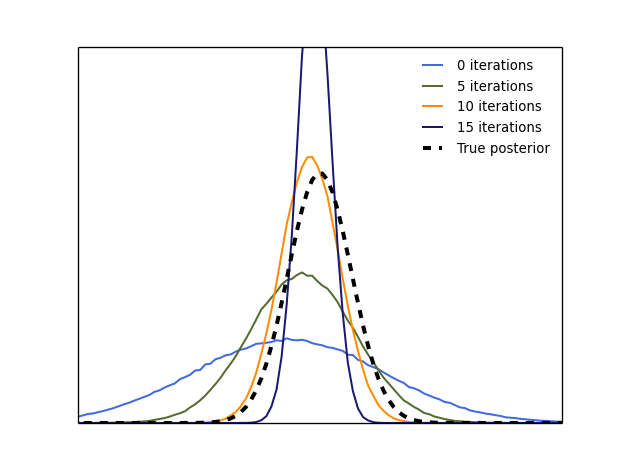
\includegraphics[width=\columnwidth]{../experiments/2015_02_28_front_page_cartoon/1/cartoon.png}
\caption{Illustration of a family of variational distributions implicitly defined by
  stochastic gradient descent. Of these, iteration 10 maximizes the lower bound on
  the marginal likelihood.}
\label{fig:cartoon}
\end{center}
\end{figure}

Optimization is an intrinsically information-destroying process. A good optimization
procedure maps any initial starting point to one or a few final optima. (keeping
track of entropy lets us know how many bits we have `learned'; one advantage of
stopping before optimization is complete is that it limits the number of bits we
can learn; given a finite amount of data we don't expect to be able to learn
more than a finite number of bits; cite reversible learning paper. Thus early
stopping is one of many ways to reduce the hypothesis space. Cite statistical
learning theory, MDL.)

In this paper, we formalize this argument with a Bayesian approach. (optimization as a series of distributions; variational
inference; marginal likelihood bound)

(Entropy and energy terms; Energy is goodness of fit to training data; entropy
is trying to force the posterior mass to spread out and avoid overfitting)

[TODO: Talk about the bridging the gap paper]

(We first show how to keep track of entropy; simple experiments illustrating the point
experiments; Then show how to keep track of entropy scaled up; How to inject
noise to be more simliar to MCMC)

\subsection{Contributions}

\begin{itemize}
\item We give a simple algorithm based on stochastic gradient descent that produces samples from a variational posterior along with an estimate of the marginal likelihood.
This algorithm, called entropic descent, performs approximate Bayesian inference in a manner analogous to Hamiltonian Monte Carlo, but without the need for accept-reject steps, and with the ability to operate on minibatches.
This allows regularization parameters to be set within a single training pass.
\item We show that the entropy of our nonparametric variational distribution can be computed exactly by a simple sum of log-momentum decay terms.
\item Early stopping can be viewed as taking a single sample from the implicitly-defined variational distribution.
Tracking the approximate marginal likelihood gives a stopping rule without a validation set.
\end{itemize}


\section{Constructing a tight variational bound}

We're trying to maximize the variational lower bound on the marginal likelihood of a model:
%
\begin{align}
\log Z & = \int q(\params) \log \pun(\params) d\params - \int q(\params) \log q(\params) d\params \nonumber \\ & \quad - \KL{p(\vv|\vx)}{q(\vv|\vx)} \\
& \geq \int q(\params) \log \pun(\params) d\params \underbrace{- \int q(\params) \log q(\params) d\params}_{\textnormal{\normalsize Entropy $H[q]$}}
%  & = \mathbb{E}_q[\log p(\params)] + H[q]
\end{align}
%
where $q(\params)$ is a variational distribution.
The two terms can be interpreted as (negative) energy and entropy terms, respectively.

We define a nonparametric variational distribution implicitly as the output of a random initialization run through $T$ iterations of stochastic gradient descent (SGD):
%
\begin{align}
\params_1, \vv_1 & \sim \distinit \\
q^{\SGD}_T(\params, \vv) & = \SGD(\stepsizes, \decays, \params_1, \vv_1, T)
\end{align}
%

\subsection{Leapfrog Dynamics}

In the limit of small step sizes $\stepsize$, leapfrog dynamics exactly preserve the energy and entropy of the system, and therefore the marginal likelihood of the implicit variational distribution remains the same.

No matter the step size, leapfrog dynamics always exactly preserve entropy.
The only time entropy is added or removed from the system is when the momentum is resampled.
The difference in this entropy is given by:
%
\begin{align}
\Delta H & = H_t' - H_t \\
 & = - \expectargs{q_(\vx)}{\expect_{q'(\vv|\vx)} \log q'(\vv|\vx) - \expect_{q(\vv|\vx)} \log q(\vv|\vx)} \nonumber \\
 & = - \expect{q_(\vx)} \Bigg[ \expect_{q'(\vv|\vx)} \log q'(\vv|\vx) - \expect_{q(\vv|\vx)} \log r(\vv|\vx) \nonumber \\ 
 & \quad - \underbrace{\expect_{q(\vv|\vx)} \log \frac{ q(\vv|\vx)}{r(\vv|\vx)}}_{\textnormal{\scriptsize $\KL{q(\vv|\vx)}{r(\vv|\vx)}$}} \Bigg] \label{eq:r slack}
\end{align}
%

In the case of SGD with momentum, entropy is lost only when drag is applied.
If the momentum is decayed by $\vv_{t+1} = \decay_t \vv_t$, then the amount of entropy lost is exactly $\log \decay$.

\begin{figure}[t]
%\vskip 0.2in
\begin{center}
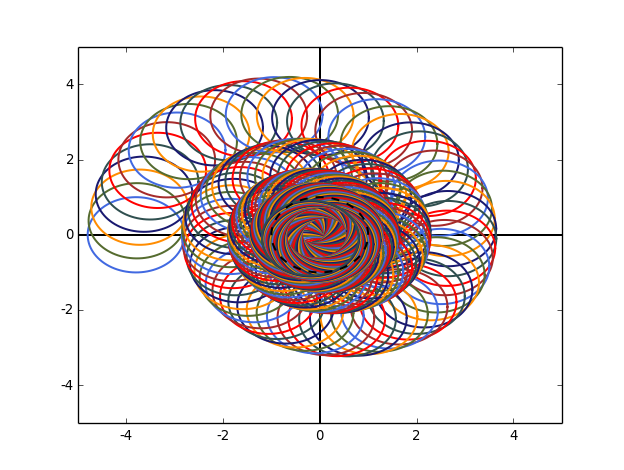
\includegraphics[width=\columnwidth]{../experiments/2015_02_23_gaussian_phase_diagrams/1/phase_diagram}
\caption{Phase diagram over time.}
\label{fig:phase}
\end{center}
\end{figure}








\begin{algorithm}
   \caption{Entropic Descent}
   \label{alg:entropic-descent}
\begin{algorithmic}[1]
	\State {\bfseries input:}
	Weight initialization scale $\sigma_0$, \\
	velocity randomization level $\decay$, \\
	annealing schedule $\stepsizes$, \\
	time step $\epsilon$, \\
	highest eigenvalue $\lambda$, \\
	negative log likelihood $L(\params, t)$
	\State initialize $\vv_1 \sim \N{0}{\vI_D}$
	\State initialize $\params_1 \sim \N{0}{\sigma_0 \vI_D}$
	\State $\entropy = \frac{D}{2} (1 + \log 2 \pi) + D \log\sigma_0 + \frac{1}{2} (D - |\vv|_2^2)$
	\For{$t=1$ {\bfseries to} $T$}
		\State $\entropy = \entropy + \frac{1}{2} |\vv|_2^2$ \Comment{Update entropy}
		\State $d =   \stepsizes_t \lambda     + (1 - \stepsizes_t) \sigma_0^2$ \Comment{Anneal stepsize}
		\State $\vg = \stepsizes_t \gradparams + (1 - \stepsizes_t) \frac{\vx}{\sigma_0^2}$ \Comment{Anneal gradient}
		\State $\vv_{t+1} = \vv_t + d \times \vg$ \Comment{Update velocity}
		\State $\params_{t+1} = \params_t + d \times \vv$  \Comment{Update position}
		\State $\entropy = \entropy - \frac{1}{2} |\vv|_2^2$  \Comment{Downdate entropy}
		\State $\vr \sim \N{0}{\vI_D}$
		\State $d\vv = \sqrt{1 - \decay^2} d\vv + \decay \vr$ \Comment{Perturb velocity}
   \EndFor
   \State \textbf{output} sample $\params_T$, estimate of entropy $\entropy$
\end{algorithmic}
\end{algorithm}

$\lambda$ is the square root of the highest eigenvalue of the Hessian of the log-posterior at the mode.
$\decay$ controls the amount velocities randomize each iteration.

Since we can sample exactly from $q$, we can approximate the first (``energy'') term of $L$ using one or more Monte Carlo samples.

The variational parameters of $q^{\SGD}$ are the learning rate schedule $\stepsizes$, the momentum decay schedule $\decays$ and the initial distribution $\distinit$.
Perhaps for now we'll set $\distinit$ to be the prior, although it could really be anything.

\subsection{The need for Annealing}
If we didn't anneal, the KL term in equation \ref{eq:r slack} wouldn't go to zero even as the step-size approached zero.

\subsection{But what about detailed balance?}

\section{Related work}


RMSprop~\cite{Tieleman2012} or Adam~\citep{Adam14}

\paragraph{MCMC for variational inference}
Our method can be seen as a special case of \citet{Bridging14}.


\paragraph{Bayesian neural networks}
Variational inference in Bayesian neural-network models such as deep Gaussian processes~\citep{deepGPVar14}.
\citet{kingma2014efficient} show how neural networks having unknown weights can be reformulated as neural networks having known weights but stochastic hidden units, and exploit this connection to preform efficient gradient-based inference in Bayesian neural networks.


\paragraph{Black-box stochastic variational inference}
\citet{alp2014blackbox} introduce a general scheme for variational inference using only the gradients of the log-likelihood of a model.
However, they constrain their variational approximation to be Gaussian, as opposed to our free-form variational distribution.

\paragraph{Adaptive learning rates for SGD}
\citet{courbariaux2014low} give a method based on Hessian-vector products to adapt learning rates for stochastic gradient descent without momentum.


\paragraph{Langevin Dynamics}
\citet{welling2011bayesian} introduced stochastic gradient Langevin dynamics for doing inference with minibatches.
\citet{ma2013estimating} use Langevin dynamics and a floating temperature to estimate partition functions of graphical models.
\citet{vollmer2015non} analyze the asymptotics of Langevin dynamics.

\paragraph{Annealed HMC}
\citet{sohl2012hamiltonian} used HMC including an accept/reject step for annealed importance sampling to estimate partition functions.

\paragraph{HMC with fewer rejections}
\citet{sohl2014hamiltonian} introduce a variant of HMC that requires fewer rejections by extending trajectories in some cases where a rejection would otherwise occur, giving a sampler that does not obey detailed balance but still samples from the correct stationary distribution.

\paragraph{MCMC with mini batches}
[TODO: more citations go here]
\citet{betancourt2015fundamental} argues that minibatches are fundamentally incompatible with HMC.


\section{Future Work and Extensions}

We could derive a variational inference algorithm based on RMSProp, and a corresponding variant of Hamiltonian Monte Carlo.

Hyperparameters typically come in two forms:
Regularization parameters and training parameters.
Optimizing marginal likelihood rather than training loss lets us set regularization parameters during training without using a validation set.
The marginal likelihood estimate lets us optimize the variational parameters (training hyperparameters) in an outer loop.
However, optimizing more than a few of these is difficult without gradients.
We could gain access to exact gradients of the variational lower bound with respect to all variational parameters by simply using reverse-mode differentiation.
\citet{MacDuvAda2015hyper} showed that this can be done in a memory-efficient way for momentum-based learning procedures.
Combining these two procedures would allow one to set all hyperparameters using gradient-based methods without the need for a validation set.

%\subsection{Acknowledgements}
%We thank Roger Grosse for helpful discussions.


[TODO: Cite Nando's variational MCMC paper]


\bibliography{references.bib}
\bibliographystyle{uai2015stylefiles/icml2015}



\end{document}



\begin{figure*}[t]
%\vskip 0.2in
\begin{center}
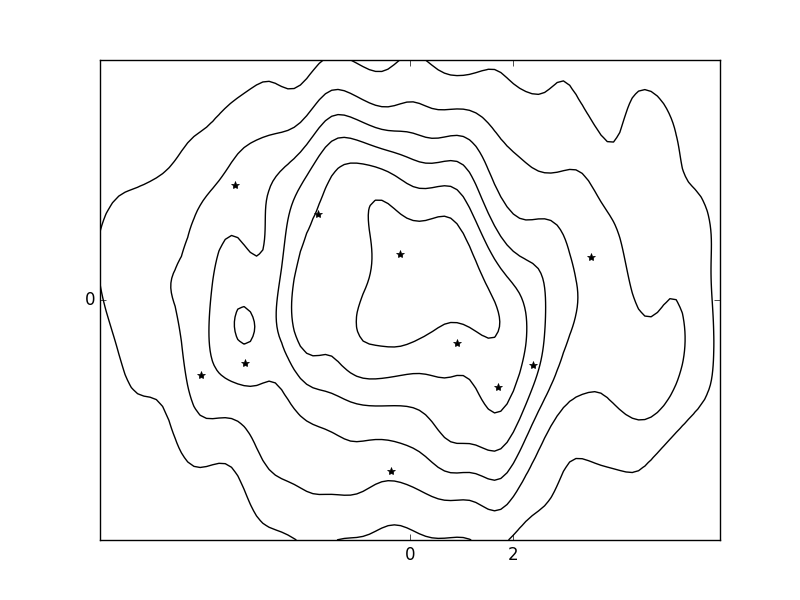
\includegraphics[width=0.18\linewidth]{../experiments/2015_02_19_caibration/5_figure/seqs/densities_0}
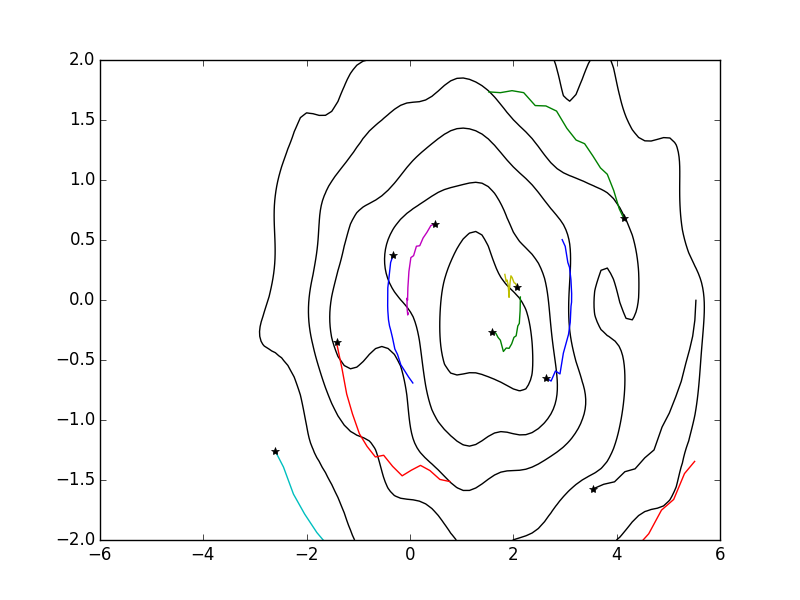
\includegraphics[width=0.18\linewidth]{../experiments/2015_02_19_caibration/5_figure/seqs/densities_200}
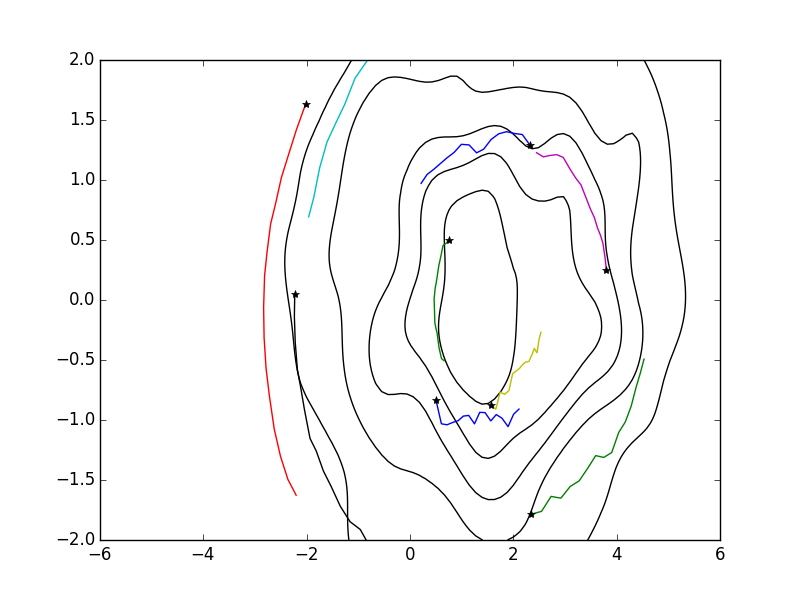
\includegraphics[width=0.18\linewidth]{../experiments/2015_02_19_caibration/5_figure/seqs/densities_400}
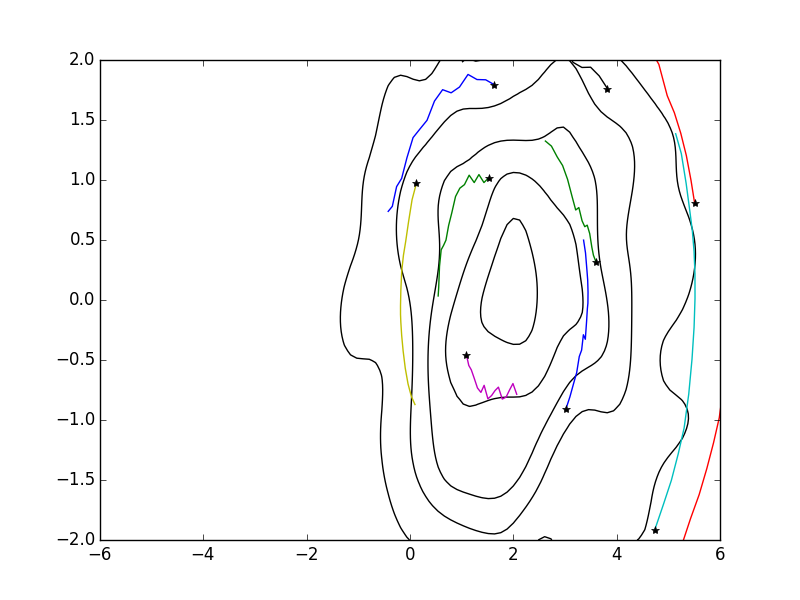
\includegraphics[width=0.18\linewidth]{../experiments/2015_02_19_caibration/5_figure/seqs/densities_600}
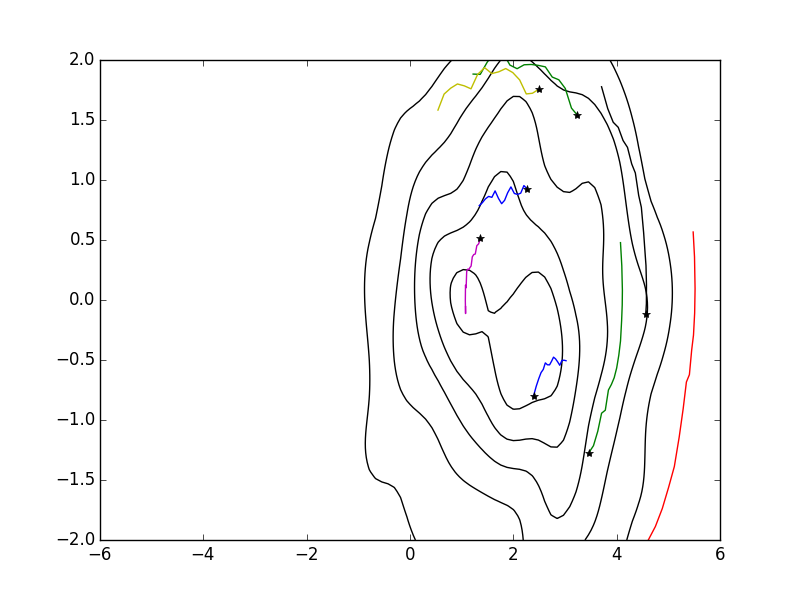
\includegraphics[width=0.18\linewidth]{../experiments/2015_02_19_caibration/5_figure/seqs/densities_800}
\caption{Left to right: Phase diagrams over time.}
\label{fig:dynamics}
\end{center}
\end{figure*}



\section{Online gradient updates of learning rate and momentum}

A simple procedure to sample from a variational posterior could look like this:
Start with $\stepsize_1 = 1$, $\decay_1 = 1$.
At each iteration of SGD, update each in the direction that would improve the bound at computed at the current step,~$L_{t+1}$:
%
\begin{align}
\vv_{t+1}     & = \decay_t \vv_t - g(\params_t) \\
\params_{t+1} & = \params_t + \stepsize_t \vv_{t+1} \\
\stepsize_{t+1} & = \stepsize_t + s_\stepsize \pderiv{L_t}{\stepsize_t} \\
\decay_{t+1} & = \decay_t + s_\decay \pderiv{L_t}{\decay_t}
\end{align}
%
where $s_\stepsize$ and $s_\decay$ are `meta' step sizes.

Which direction do these gradients point?
For $\stepsize$,
%
\begin{align}
\pderiv{L_t}{\stepsize_t} = g(\params_{t+1}) \vv_{t+1}
\end{align}
%
which means that the learning rate will increase as long as the gradient is pointing in the same direction as the velocity.
It also has the effect of going at the same speed when the gradient becomes small.
This is what we want:  If learning stopped when the gradient was zero, then the optimizer would converge.

For $\decay$, the gradient has the form:
%
\begin{align}
\pderiv{L_t}{\decay_t} = - g(\params_{t+1}) \vv_{t} \stepsize_t - \log \decay_t
\end{align}
%
The first term is exactly the same as our heuristic, scaled by $\stepsize$!
It will increase the velocity if the gradient points in the opposite direction from the velocity.

The second term has a damping effect:  If the gradient, velocity, or stepsize are all small, then this term will try to set the momentum decay term to 1.
When the momentum decay term is exactly one, no entropy is lost or gained by the optimizer.










How to optimize the variational parameters $\stepsizes$ and $\decays$?
Keep in mind that these could be different for every iteration of SGD as well as every parameter.
Keep in mind that since our approximation to the lower bound is deterministic in $\stepsizes$ and $\decays$, we can easily ``overfit'' the variational hyperparameters unless we average over multiple runs of SGD. [TODO: this doesn't have to be the case. It depends on whether we can reversibly infer the momentum decay rate as we go along.]

\section{Online gradient updates of learning rate and momentum}

A simple procedure to sample from a variational posterior could look like this:
Start with $\stepsize_1 = 1$, $\decay_1 = 1$.
At each iteration of SGD, update each in the direction that would improve the bound at computed at the current step,~$L_{t+1}$:
%
\begin{align}
\vv_{t+1}     & = \decay_t \vv_t - g(\params_t) \\
\params_{t+1} & = \params_t + \stepsize_t \vv_{t+1} \\
\stepsize_{t+1} & = \stepsize_t + s_\stepsize \pderiv{L_t}{\stepsize_t} \\
\decay_{t+1} & = \decay_t + s_\decay \pderiv{L_t}{\decay_t}
\end{align}
%
where $s_\stepsize$ and $s_\decay$ are `meta' step sizes.

Which direction do these gradients point?
For $\stepsize$,
%
\begin{align}
\pderiv{L_t}{\stepsize_t} = g(\params_{t+1}) \vv_{t+1}
\end{align}
%
which means that the learning rate will increase as long as the gradient is pointing in the same direction as the velocity.
It also has the effect of going at the same speed when the gradient becomes small.
This is what we want:  If learning stopped when the gradient was zero, then the optimizer would converge.

For $\decay$, the gradient has the form:
%
\begin{align}
\pderiv{L_t}{\decay_t} = - g(\params_{t+1}) \vv_{t} \stepsize_t - \log \decay_t
\end{align}
%
The first term is exactly the same as our heuristic, scaled by $\stepsize$!
It will increase the velocity if the gradient points in the opposite direction from the velocity.

The second term has a damping effect:  If the gradient, velocity, or stepsize are all small, then this term will try to set the momentum decay term to 1.
When the momentum decay term is exactly one, no entropy is lost or gained by the optimizer.

Taken together, these two update rules mean that when the local gradient goes to zero, the velocity will stabilize and not go to zero, and the stepsize will also remain constant.
This is also necessary for the optimizer not to stop at local minima.
These dynamics will also skate over basins at a constant speed, which is what we want.

[TODO] see if there are any other steady states of this system, such as going in a circle around the minimum of a parabola.

No burn in!

\section{Reversibility}

We can probably play with the order of the SGD steps to make them reversible.
But do we need to?
If we interpret $\stepsizes$ and $\decays$ as just variational parameters, then they are "outside" the system, and the only way they can go wrong is by failing to find a good bound, or by messing up our estimates of the bound.

\section{Alternative approach - decay rate from velocity variance estimate}

If we treat $\decays$ as variational parameters we have to use the same
$\decays$ regardless of starting position and trajectory. Some smoothing will
therefore be necessary to avoid overfitting to a perticular trajectory. If we
evaluate multiple trajectories from an ensemble of starting positions, we can
chose $\decay$ based on the statistical properties of this ensemble.

In particular, we happen to know the target distribution's marginal distribution
over $\vv$ (it's just $N(0, 1)$ independent of $\params$).  The purpose of the
decay term is to collapse the velocity towards this distribution.  We can
estimate the variance, $\sigma_v^2$, of the variational distribution over $\vv$
at time $T$ using the ensemble and then, for example, choose:
\begin{align}
\log \decay = - \beta_0 \log \sigma_v
\end{align}
For some overall ``decay speed'' $\beta_0$. [TODO: think about the multivariate
case, in which $\decays$ could be a matrix. With $N << D$ samples, we can't
hope to estimate the full covariance matrix. Maybe some ones on the diagonal
would help.]

\section{Alternative approach - decay rate adapted using curvature information}

If we base $\decays$ entirely on $\params$ and not on $\vv$ we can have
different $\decays$ for different trajectories and we don't have to worry about
overfitting.

If we have a good estimate of the entropy difference between initial and target
distributions we can choose some integrable $\decays$ schedule that amortizes
the entropy change over multiple steps. The log determinant of the Hessian is
such an estimate. It's exact in the Gaussian case and hopefully a reasonable
approximation otherwise. Looking at the individual eigenvalues of the Hessian
gives a way to estimate the required entropy injection/extraction along each
eigendirection.

[TODO: think about how to avoid actually diagonalizing the Hessian]

[TODO: think about how to handle negative eigenvalues]

\section{Yet another approach - velocity randomization}

An orthonormal transformation of the velocity vector leaves the target
distribution invariant and the entropy unchanged. So if we just apply a
transformation of $I + \alpha T$ at each iteration, we will get a similar effect
to that of a per-parameter $\decay$, without having to devise an elaborate
heuristic to assign a $\decay$ to each parameter. There is just one global
$\decay$ which controls the overall rate of entropy extraction and the remaining
entropy is automatically distributed among the parameters as needed by the
random rotations.

This is a lot like randomizing velocities in the manner of HMC, except that it
doesn't add or remove any net entropy. Entropy is only added or removed when we
apply $\decay$ for which we are rewarded or penalized as appropriate.

------

Since we can sample exactly from $q$, we can approximate the first (``energy'') term of $L$ using one or more Monte Carlo samples.
We can compute the second (``entropy'') term exactly:
\begin{align}
H[q_t] = H[q_0] - \sum_{t=1}^{T} \sum_{d=1}^{D} \log \decay_{td}
\end{align}
%
where $f(\params)$ is the negative log-likelihood and $\decay_{td}$ is the velocity decay rate for step $t$ and parameter $d$.
[Maybe: mention that it's only a lower bound on the entropy in the case of finite precision.]
